\documentclass{nature3}
\usepackage{graphicx}
\usepackage{float}
\usepackage{verbatim}
\usepackage{hyperref}
\usepackage{amsmath}
\usepackage{amssymb}
\usepackage{aas_macros_nature}
\usepackage{lineno}
\usepackage{caption}

\linespread{1.0}
\linenumbers % turn line numbering on or off

\newcommand{\starname}{TIC 141146667}

\newcommand{\farcm}{\mbox{\ensuremath{.\mkern-4mu^\prime}}}%    % fractional arcminute symbol: 0.'0
\newcommand{\farcs}{\mbox{\ensuremath{.\!\!^{\prime\prime}}}}%  % fractional arcsecond symbol: 0.''0

\newcommand{\kms}{\ensuremath{\rm km\,s^{-1}}}
\newcommand{\ms}{\ensuremath{\rm m\,s^{-1}}}

\renewcommand*{\thefootnote}{\fnsymbol{footnote}}

%%%%%%%%%%%%%%%%
% INSTITUTIONS %
%%%%%%%%%%%%%%%%
\newcommand{\carnegie}{Observatories of the Carnegie Institution for Science, Pasadena, CA 91101, USA}
%%%%%%%%%%%%%%%%

%%%%%%%%%%
% VALUES %
%%%%%%%%%%
% NOTE: might need to be ingested before submission 
\newcommand{\stteff}{YYYY}
\newcommand{\stagemyr}{40}
\newcommand{\periodhr}{3.930}


%%%%%%%%%%%%%%%%%%%%%%%%%%%%%%%%%%%%%%%%%%
%%%%%%%%%%%%%%%%%%%%%%%%%%%%%%%%%%%%%%%%%%

\title{A Plasma Torus Around a Young Low-Mass Star}

\begin{document}

\author{Luke G. Bouma$^{1,2}$}

\maketitle

\scriptsize
\begin{affiliations}
\item \carnegie
\item Carnegie Fellow
\end{affiliations}
\normalsize

%%%%%%%%%%%%%%%%%%%%%%%%%%%%%%%%%%%%%%%%%%%%%%%%%%%%%%%%%%%%%%%%%%%%%%%%%%%%%%%
%%%%%%%%%%%%%%%%%%%%%%%%%%%%%%%%%%%%%%%%%%%%%%%%%%%%%%%%%%%%%%%%%%%%%%%%%%%%%%%

\begin{abstract}
\normalfont
Roughly one percent of red dwarfs younger than 100 million years
show structured, periodic optical light curves suggestive of
transiting opaque material that corotates with the star
\cite{Rebull2016,Stauffer2017,Rebull2018,Bouma2024}.  The
composition, origin, and even the existence of this material are
uncertain. The main alternative hypothesis is that these complex
periodic variables (CPVs) are explained by complex distributions of
bright or dark regions on the stellar surfaces
\cite{Koen2021}.  Here, we present time-series spectroscopy and
photometry of a rapidly-rotating ($P$=3.9\,hr)
CPV, TIC~141146667. The spectra show coherent sinusoidal Balmer
emission at twice to four times the star's equatorial velocity,
demonstrating the existence of extended clumps of circumstellar
plasma --- a plasma torus.  Given that long-lived condensations of
cool ($10^4$ K) plasma can persist in the hot ($10^6$ K) coronae of
stars with a wide range of masses
\cite{CollierCameron1989,Townsend2005,Dunstone2006,Petit2013,Waugh2022,Daley-Yates2024},
these data support the idea that around the lowest-mass stars, such
condensations can be optically thick; the exact origin of the
material and its microphysical opacity remain unclear.
\end{abstract}

\maketitle

%%%%%%%%%%%%%%%%%%%%%%%%%%%%%%%%%%%%%%%%%%%%%%%%%%%%%%%%%%%%%%%%%%%%%%%%%%%%%%%
%%%%%%%%%%%%%%%%%%%%%%%%%%%%%%%%%%%%%%%%%%%%%%%%%%%%%%%%%%%%%%%%%%%%%%%%%%%%%%%

% Main text – up to 3,000 words, excluding abstract, Methods,
% references and figure legends.

\section{Main}
\label{sec:main}

%\subsection{Introduction}
M dwarfs, stars with masses below about half that of the Sun, are the
only type of star to offer near-term prospects for detecting the
atmospheres of rocky exoplanets with surface water
\cite{NAP26141}.  Investment with JWST has proceeded accordingly.  How
an M dwarf's evolution influences its planets---especially the
retention of their atmospheres--- has concurrently become a major
theme in exoplanet and stellar astrophysics.  Previous work has
established that most M dwarfs host close-in planets
\cite{Dressing2015} that are often subject to long
circumstellar disk lifetimes \cite{Ribas2015}, to large doses of UV
radiation \cite{France2013}, and to a high incidence of flares and
coronal mass ejections \cite{Gunther2020}.  However, despite excellent
work in these areas, the properties of the plasma and magnetospheric
environments that bathe young, close-in exoplanets have remained
challenging to quantify.

One glaring example of our current ignorance is the complex periodic
variables (CPVs).  While Figure~\ref{fig:lc} highlights the main object of
interest in this article, over one hundred analogous objects have
now been found by K2 and TESS 
\cite{Rebull2016,Stauffer2017,Rebull2018,Zhan2019,Rebull2020,Bouma2024}.
These CPVs are
phenomenologically identified based on their highly structured and
periodic optical light curves;
most are M dwarfs with rotation periods shorter than two days.
Within current sensitivity limits, none have primordial disks
\cite{Stauffer2017,Bouma2024}.
However, $\approx$3\% of stars a few million years old show this
behavior, and the observed fraction decreases to $\approx$0.3\%
by $\approx$150\,Myr \cite{Rebull2020}.

The two leading hypotheses to explain the CPVs are either that
transiting clumps of circumstellar material corotate with the star
\cite{Stauffer2017,Gunther2022,Bouma2024}, or that these stars represent
an extreme in naturally-occurring distributions of starspots or faculae
\cite{Koen2021}.  
% TODO: might want to plug Shapiro, Seager, ACC dark faculae...
While the main argument against a starspot-only explanation invokes the
timescales and amplitudes of the sharpest photometric features, no
independent evidence has yet been acquired for the presence of any
circumstellar material.  Geometrically, transiting clumps would imply an
occurrence a few to at most ten times the observed rate.  The clumps
could therefore exist around 10-30\% of M dwarfs during their early
lives.


\begin{figure}[!t]
  \centering
  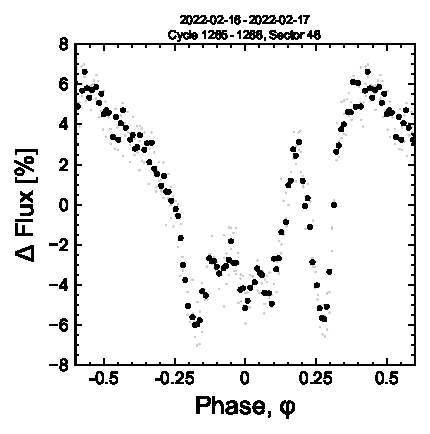
\includegraphics[width=0.7\textwidth]{figures/f1.pdf}
  \captionsetup{labelformat=empty}
  \caption{{\bf Figure 1 (Movie):  TIC~141146667 is a complex periodic
  variable (CPV).}  The online movie,
  available
  \href{https://lgbouma.com/movies/TIC141146667_20250116.mp4}{here},
  shows a baseline of 5{,}784 cycles irregularly sampled over three
  years.  The TESS light curve is phased to the \periodhr\ hour period in
  groups of a few cycles per frame.  This is the period both of
  stellar rotation, and (we hypothesize) of corotating clumps of
  circumstellar material.  Raw data acquired with two minute sampling
  are in gray; black averages to 100 points per cycle.  Similar to
  other stars of this class, the sharp photometric features persist
  for tens to thousands of rotational cycles. }
  \label{fig:lc}
\end{figure}


The dearth of evidence for circumstellar material around CPVs is
surprising given that separate studies of young stars have, for
decades, reported that stellar coronae contain both hot ($10^6$ K) and
cool ($10^4$ K) plasma. In particular, time-series spectroscopy for
stars with a wide range of masses has shown periodic high-velocity
absorption and emission in Balmer lines such as H$\alpha$, interpreted
as long-lived, corotating clumps of cool plasma
\cite{CollierCameron1989,Donati2000,Dunstone2006,Skelly2008}.
Such clumps are forced into corotation by the magnetic field, and the
exact geometry of where the plasma can accumulate is dictated by the
field's topology.  For instance, a tilted dipole field tends
to yield an accumulation surface of a warped torus
\cite{Townsend2005}, whereas in the limit of a single strong field
line, accumulation occurs at the line's apex, furthest from the star
\cite{Waugh2022}.
To date, none of these spectroscopic variables have shown any
photometric anomalies \cite{Bouma2024}, leaving open the issue of
whether they are related to CPVs.
%A circumstantial argument that they might is that CPVs do respond to
%sudden magnetic field changes: the otherwise long-lived eclipse
%features often disappear following stellar flares
%\cite{Stauffer2017,Bouma2024}.

In this study, we present the first observations of corotating clumps of
cool plasma around a CPV.  We identified TIC~141146667 in previous work
\cite{Bouma2024} by searching the TESS two-minute data \cite{Ricker2015}
for stars showing at least three sharp, periodic dips per cycle.  We
selected the star for spectroscopy because its brightness and rapid
rotation enable efficiently studying small variations in the line profiles.  We
observed for five hours on 17~February~2024 (UT) using the High
Resolution Echelle Spectrometer (HIRES; \cite{vogt_hires_1994}) on the
Keck I 10m telescope.  TESS observed the star over a four week period
from 30~January~2024 to 26~February~2024 with a duty cycle of 77\%.
During the spectral observations, TESS was performing a data downlink;
TESS data collection resumed 12 hours (three rotation cycles) after the
spectra were acquired.  Extended Data Figure~\ref{fig:fulllc} shows the
detailed photometric behavior of the star before and after the exact
epoch of observation; the photometric morphology is similar before and
after the data gap.


\section{Results}

\begin{figure}[!tp]
  \centering
  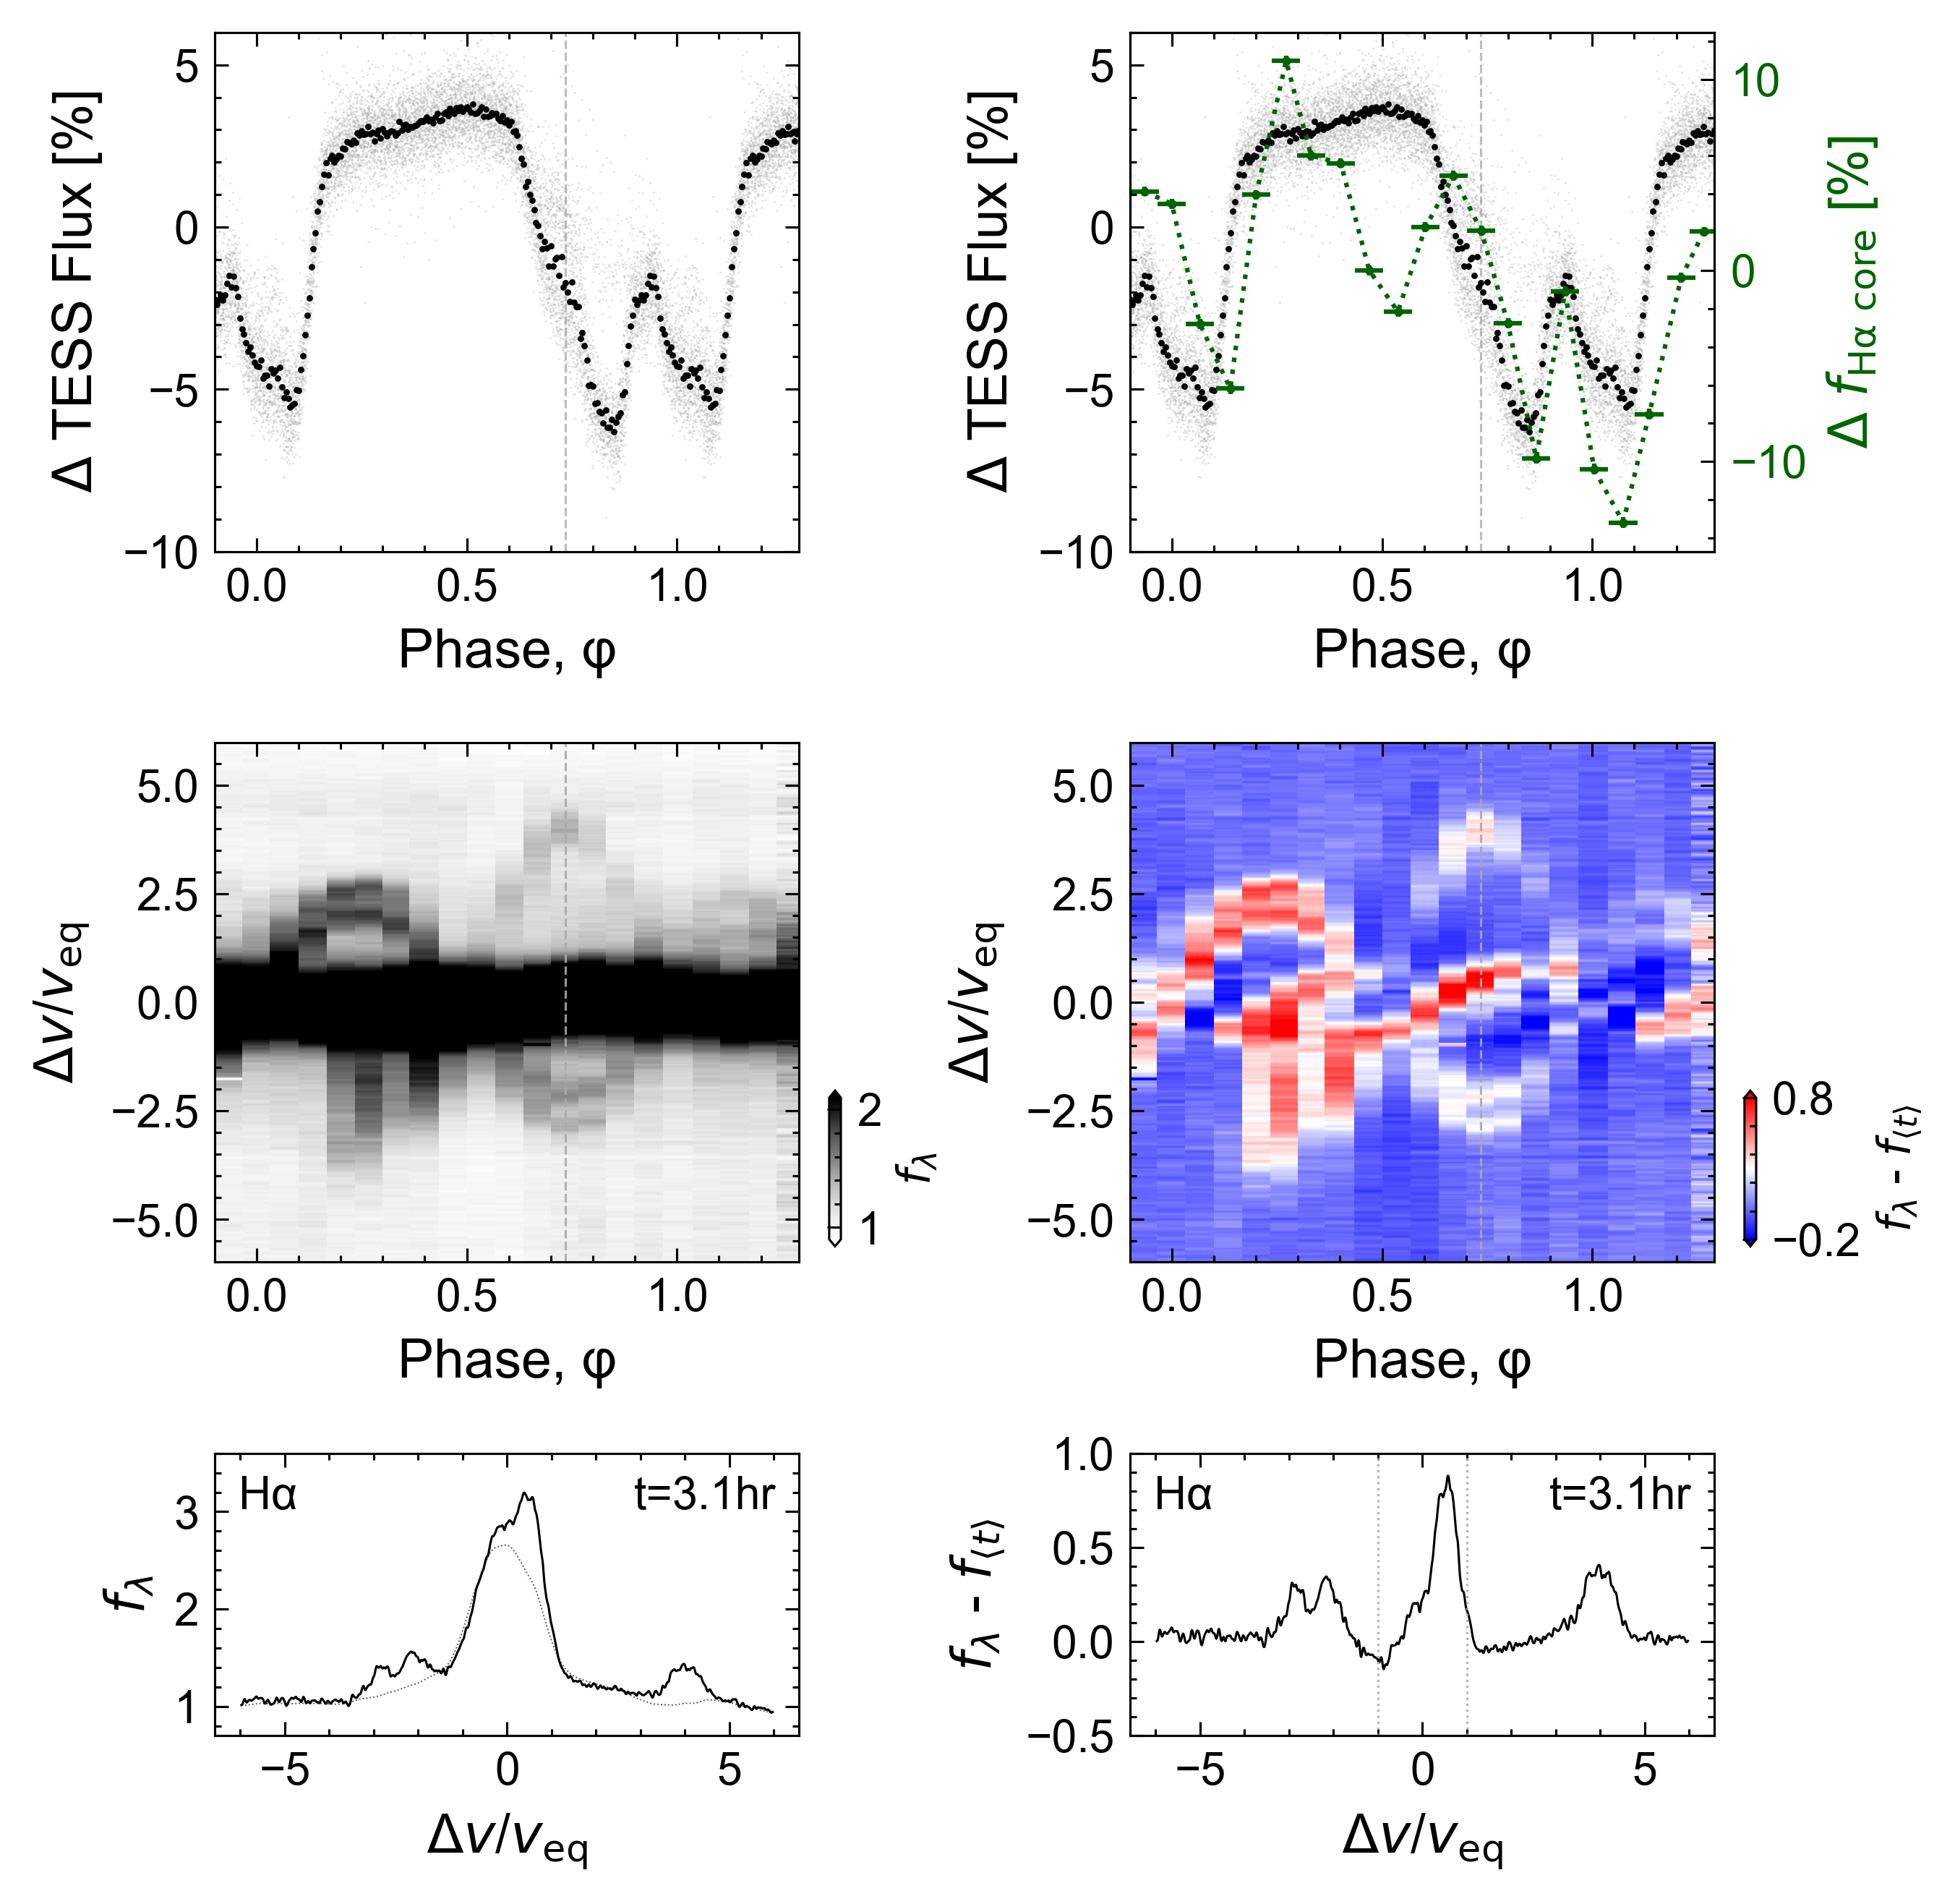
\includegraphics[width=0.99\textwidth]{figures/f2.png}
  \captionsetup{labelformat=empty}
  \caption{{\bf Figure 2 (Movie):}  
  Hydrogen emission from circumstellar plasma orbiting TIC 141146667.
  {(\bf TODO)}For the best experience, please view the online movie
  available
  \href{https://lgbouma.com/movies/TIC141146667_sixpanel.mp4}{here}.
  {\bf Panel a:} TESS light curve from 5 February 2024 to 26 February
  2024 (UT) folded on the \periodhr\ hour period.  Black points are
  phase-averaged; gray are the raw data.
  {\bf Panel b:} Keck/HIRES H$\alpha$ spectra
  acquired on UT 17 February 2024.  The continuum is set to unity, and the
  darkest color is at twice the continuum to accentuate emission
  outside the line core ($|v/v_{\rm eq}|>1$, for $v_{\rm eq}$=130\,\kms).
  While emission in the line core originates in the stellar
  chromosphere, the sinusoidal emission features are most readily
  described by a warped plasma torus.
  {\bf Panel c:} Individual epochs of Panel b, visible in the
  online movie.  The dotted line shows the time-averaged spectrum,
  $f_{\langle t \rangle}$.
  {\bf Panel d:} As in Panel a, but overplotting the
  median-normalized H$\alpha$ light curve at $|v/v_{\rm eq}|<1$.
  {\bf Panel e:} As in Panel b, after subtracting the time-averaged
  spectrum. In addition to circumstellar emission, the line core shows
  absorption during the plasma clump transits.  The asymmetric stretch
  is set to match the dynamic range of the data.
  {\bf Panel f:} Individual epochs of Panel e, visible in the online
  movie.}
  \label{fig:spec}
\end{figure}

% photometry
Figure~\ref{fig:spec} shows the data from February 2024.  Over
timescales of years, CPVs maintain a fixed period while their
photometric morphology evolves.  TIC~141146667 indeed evolved relative
to the February 2022 discovery data \cite{Bouma2024}.  In February
2024, the average photometric signal showed a small brightening
over 45\% of the period, followed by a complex flux dip spanning 55\%
of the period.  This eclipse feature shows two to three local
photometric minima, and one to two local maxima.  Its W-shape is
suggestive of eclipse geometries seen in some forward models of warped
plasma tori \cite{Townsend2008}.

% ** keck/hires: emission beyond v/veq>1
The spectroscopy shows emission beyond the star's equatorial velocity
($v_{\rm eq}$=130\,\kms).  There are at least two distinct emission
components, separated by half a cycle in phase.  The first component
has clearer sinusoidal behaviour and is double-peaked, with peak
semi-amplitudes of $K_1$=2.1\,$v_{\rm eq}$ and 2.7\,$v_{\rm eq}$.
There is significant non-periodic variability in the emissivity of
this double-peaked component: the flux excess begins with an amplitude
of 70\% of the continuum flux early in the observation sequence, and
diminishes to 10\% by its end.  The component 180$^\circ$ opposite in
phase is detected only from $\phi$=0.2-1.0.  From $\phi$=0.2-0.5, this
latter component appears connected to the star in velocity space.
While its peak semi-amplitude of $K_1$=3.9\,$v_{\rm eq}$ is achieved
at both $\phi$=0.25 and 0.75, its amplitude similarly decreases from a
60\% excess over the continuum at the beginning of the observation
sequence to a 10\% excess by its end.  The sinusoidal period for all
of these emission components is consistent with the photometric
\periodhr\ hour period.  

These sinusoidal emission features require circumstellar clumps of
partially-ionized hydrogen to corotate with the star.  
Based on the period, this material's motion is not Keplerian; it can
only be explained by plasma being dragged along with the rotating
stellar magnetic field. 
The velocity semi-amplitude of the sinusoids gives the distance
of the clumps from the stellar surface: 2.1-2.7\,$R_\star$ for the
closer clump, and 3.9\,$R_\star$ for the other.   These clumps transit
in front of the star when passing from negative to positive velocity.
This implies that the spectroscopic transit of the 2.1-2.7\,$R_\star$
clump occurs simultaneously with the sharp photometric spike visible
in the TESS data.

% * keck/hires: behavior at v/veq<1
The behavior within the stellar H$\alpha$ line core, at $|\Delta v /
v_{\rm eq}|<1$, is more complex than outside it.  For stars of
this age and spectral type, one would expect emission in the line core
to be generated in the stellar chromosphere
and then modulated by any occulting material capable of absorbing or
emitting H$\alpha$ photons.  In Figure~\ref{fig:spec}e, the behavior from
$\phi$=0.4-1.2 has a simple interpretation: from $\phi$=0.4-0.9, a hot
region first gradually crosses the stellar line profile, followed from
$\phi$=0.7-1.2 by the transit of a cool region.  Phases $\phi$$<$0.4
show a mix of similar events, though the time sampling is
sufficiently coarse that the interpretation is less clear.  A final
exercise to quantify the behavior in the line core is shown in
Figure~\ref{fig:spec}d, where $f_{\rm H\alpha\ core}$ denotes the
summed flux at $|\Delta v / v_{\rm eq}|<1$.  This panel shows that
changes in the line core flux are usually correlated with the
broadband variability, except at $\phi$=0.5, during the transit of the
3.9\,$R_\star$ clump and the occultation of the lower-velocity clump.

\begin{table*}
\scriptsize
\setlength{\tabcolsep}{2pt}
\centering
\caption{Selected System Parameters for TIC~141146667}
\label{tab:params}
\begin{tabular}{llcc}
\hline \hline
Parameter & Description & Value & Source\\
\hline 
%
$T_{\rm eff}$\dotfill                   & Effective Temperature (K) \hspace{9pt}\dotfill                 & 2972 $\pm$ 40    & 1 \\
%
%$\log{g_{\star}}$\dotfill              & Surface Gravity (cgs)\hspace{9pt}\dotfill                      & YYY              & X \\
%
$R_\star$\dotfill                       & Stellar radius ($R_\odot$)\dotfill                             & 0.42$\pm$0.02    & 1 \\
%
Age                                     & Stellar age range (Myr)\dotfill                                & 35-150  & 2 \\
%
$M_\star$\dotfill                       & Stellar mass ($M_\odot$)\dotfill                               & 0.22$\pm$0.02  & 3 \\
%
$\gamma$\dotfill                        & Systemic radial velocity (\kms)\dotfill                        & 0.61 $\pm$ 1.47  & 4 \\
%
Spec. Type\dotfill                      & Spectral Type\dotfill                                          & M5.5Ve           & 4 \\
%
$P_{\rm rot}$\dotfill                   & Rotation period (hr)\dotfill                                   & $3.930\pm 0.001$ & 5 \\
%
$v_{\rm eq}$\dotfill		                & Equatorial velocity \dotfill                                   &  130$\pm$4       & 6 \\
                                        & \hspace{3pt} ($2\pi R_\star/P_{\rm rot}$) (\kms)	             &                      \\
%
$v_{\rm eq}\sin{i_\star}$\dotfill		    & Projected rotational\dotfill                                   &  138$\pm$8       & 4 \\
                                        & \hspace{3pt} velocity (\kms)	                                 &                      \\
%
$i_\star$\dotfill                       & Stellar inclination\dotfill                                    & 	$>$63           & 4 \\
                                        & \hspace{3pt}  2$\sigma$ lower limit (deg)	                     &                      \\
%
$d$\dotfill                             & Distance (pc)\dotfill                                          & $57.54 \pm 0.09$   & 7 \\
%
$R_{\rm c}$\dotfill		                  & Keplerian corotation\dotfill
  & $1.82 \pm 0.10$  & 6 \\
                                        & \hspace{3pt} radius ($R_\star$)	                               &                      \\
%
$a_1$\dotfill                           & Clump 1 orbital radius ($R_\star$)\hspace{9pt}\dotfill         &  2.1-2.7         & 4 \\
$a_2$\dotfill                           & Clump 2 orbital radius ($R_\star$)\hspace{9pt}\dotfill         &  3.9             & 4 \\
%
$\langle$EW$_{\rm H\alpha}$$\rangle$    & Time-averaged H$\alpha$ line core                              &  X.X             & Y \\ 
                                        & \hspace{3pt} equivalent width (\AA)	                           &                      \\
Range(EW$_{\rm H\alpha}$)$_1$           & H$\alpha$ equiv. width range                                   &  X.X             & Y \\ 
                                        & \hspace{3pt} from Clump 1 (\AA)	                               &                      \\
Range(EW$_{\rm H\alpha}$)$_2$           & H$\alpha$ equiv. width range                                   &  X.X             & Y \\ 
                                        & \hspace{3pt} from Clump 2 (\AA)	                               &                      \\
\hline
\end{tabular}
\begin{flushleft}
\footnotesize{ \textsc{NOTE}---
$^*$ Given only $v\sin i$ and $2\pi R_\star/P_{\rm rot}$, $\cos i=0.11^{+0.11}_{-0.08}$.
Provenances are:
1: SED fit \cite{Bouma2024}.
2: Gaia DR3 photometry and lack of lithium (see~\ref{subsec:stparams}).
3: PARSEC v1.2S \cite{Chen2014}.
%$^6$Cluster isochrone (MIST adopted; PARSEC compared for quoted
%  uncertainty),
4: Keck/HIRES.
5: TESS light curve.
6: Derived quantity.
7: Gaia DR3 geometric \cite{GaiaDR3}.
%  3: HIRES spectra and specmatch(?),
%$^8$Pre-main-sequence CAMD interpolation (Section~\ref{sec:camd}),
}
\end{flushleft}
\vspace{-0.5cm}
\end{table*}



\section{Discussion}
% argue: how does this clarify wider phenomenology?  what general
% conclusions can be drawn?

Spectra of magetically-active, rapidly rotating stars with a wide range
of masses have been known to exhibit both sinusoidal emission features
\cite{Donati2000,Townsend2005,Dunstone2006,Skelly2008} as well as
transient absorption features in their line cores
\cite{CollierCameron1989,CollierCameron1992,Cang2020} similar to
Figure~\ref{fig:spec}.  No such stars were previously known to show
complex light curves \cite{Bouma2024}.   One interpretation for
such spectroscopic variability comes from an analogy to quiescent solar
prominences, which are cool condensations of plasma in the solar corona
that can last days to weeks \cite{VialEngvold2015}.  In our Sun's
magnetosphere, these condensations fall back to the solar surface
because gravity is stronger than any magnetic tension or centrifugal force
capable of sustaining them.  However for stars with magnetospheric radii
$R_{\rm m}$ that exceed their corotation radii $R_{\rm c}$, the
effective potential experienced by a charged particle can have a local
minimum outside $R_{\rm c}$, enabling the material to accumulate over
much longer timescales \cite{Petit2013,Daley-Yates2024}.  Generally
speaking, such material need neither transit, nor be optically thick.

Our Keck/HIRES observations are the first reported time-series
spectra of a CPV, and they show that corotating circumstellar plasma clumps 
are present in at least one such star.
Characteristic densities and masses of these
%TODO check; quote N_H instead...
clumps are $n \sim 10^{10}$\,cm$^{-3}$ and $M \sim 10^{14}$\,kg (see
Supplementary Methods Section~\ref{subsec:model}), a similar density to
solar prominences, but ten to one hundred times more massive.  This
observation rules out a ``starspot-only'' origin scenario for CPVs,
\cite{Koen2021} since such scenarios have no means of explaining
spectroscopic emission beyond the stellar disk.  Similarly, scenarios in
which the circumstellar material is made only of dust are also ruled
out.  While dust may be present, to explain the H$\alpha$ emission the
clumps must include plasma with a significant population of hydrogen
atoms in the $n$=3 excited state.  While this plasma is undoubtedly
sculpted by the star's magnetic field, it could plausibly originate from
three sites: the star, an old and undetected disk, or outgassing rocky
bodies.  This latter possibility would render CPVs as extrasolar analogs
of the Jupiter-Io plasma torus (e.g.~Ref.~\cite{Bagenal1981}).

The other potential analog for the CPVs are the $\sigma$~Ori~E
variables, a rare subset of B stars with radiatively-driven winds that
accumulate into warped plasma tori \cite{Townsend2005,Townsend2008}.
These tori tend to have dense antipodal accumulations of plasma sculpted
by tilted-dipole magnetic fields, and the transits of these clumps are
thought to produce the observed broadband photometric variability
through bound-free scattering \cite{Townsend2005} and Thomson scattering
\cite{Berry2022}.  For $\sigma$~Ori~E and almost all of its analogs, the
result is light curves that appear ``simple'', resembling those of
eclipsing binaries \cite{Townsend2008}.  The two known exceptions,
HD~37776 and HD~64740, show complex light curves resembling CPVs
\cite{Mikulasek2020,Bouma2024} and have spectropolarimetric magnetic
field maps indicating strong contributions from higher-order magnetic
moments \cite{Kochukhov2011,Shultz2018}.  There are two implications:
first, the complexity of CPVs may be a direct consequence of magnetic
fields with highly multipolar contributions.  Second, CPVs can be a
source of astrophysical false positives in photometric searches for
eclipsing binaries and transiting exoplanets around young pre-main
sequence M dwarfs \cite{Johns-Krull2016,Bouma2020}.

Pressing issues for future work include determining the composition and
origin of the circumstellar material, understanding the exact role of
the stellar magnetic field, and exploring the implied space weather
experienced by the close-in rocky exoplanets that, statistically
\cite{Dressing2015}, are likely to be present in most CPV systems.

The material's composition -- either pure plasma, or else a dusty plasma
-- can be clarified by time-series optical and infrared
spectrophotometry.  While observations of CPVs in the optical have
previously suggested chromaticity consistent with dust
\cite{Tanimoto2020,Gunther2022,Koen2023}, a gray opacity source such as
electron scattering in a plasma transiting over starspots might also
produce chromatic features \cite{Rackham2018}.  The composition and size
distribution of any dust that is present could be determined
by measuring the extinction curve for one or more CPVs from
1-10\,$\mu$m.  Composition and size distributions similar to debris from
rocky bodies seen around white dwarfs \cite{Reach2009} would indicate a
rocky-body origin.  Compositions and sizes similar to the ISM would be
indicative of condensed dust in an M dwarf wind, similar to that formed
in the environments of more evolved stars \cite{Marigo2008}.

The role of the star's magnetic field could be better understood through
new observations, and new theory.  From the theoretical perspective,
there is an urgent need for rigid-field (magneto)-hydrodynamic modeling
to go beyond previous work \cite{Townsend2005,Townsend2008} and to
explore the effects of non-dipolar field contributions.  In particular,
dynamo simulations of fully-convective M dwarfs have suggested that
global-scale mean fields might be confined to a single hemisphere
\cite{Brown2020}; such fields could yield accumulation surfaces quite
different from those that have previously been explored
\cite{Townsend2008}.  Observationally, spectropolarimetry has the
potential to assess both the field strength and topology.  An
independent probe could also be connected the recent work
\cite{Kaur2024} showing that CPVs are variable radio emitters with
emission components that can be not only persistent, but also
short-lived and highly polarized.  In particular, detecting radio
emission produced by an electron cyclotron maser instability
\cite{Callingham2021} would provide a measurement of the field
strength at the site of the emitting region.


It is currently unclear what, if any, relationship CPVs have to the
close-in rocky exoplanets that exist around most M dwarfs \cite{Dressing2015}.
However, 0.3-3\% of young M dwarfs show the CPV phenomenon
\cite{Rebull2020}, and our data show that the phenomenon occurs when
clumps of circumstellar material transit the star.  The implied
geometric correction suggests that an appreciable minority (10-30\%) of
young M dwarfs -- the rapidly rotating ones with centrifugal
magnetospheres -- host similar circumstellar environments to the CPVs.




%%%%%%%%%%%%%%%%%%%%%%%%%%%%%%%%%%%%%%%%%%%%%%%%%%%%%%%%%%%%%%%%%%%%%%%%%%%%%%%
%%%%%%%%%%%%%%%%%%%%%%%%%%%%%%%%%%%%%%%%%%%%%%%%%%%%%%%%%%%%%%%%%%%%%%%%%%%%%%%

\newpage
\begin{methods}

\renewcommand{\figurename}{Extended Data Figure}
\renewcommand{\tablename}{Extended Data Table}
\setcounter{table}{0}  
\setcounter{figure}{0}  

\subsection{Observations \& Data Reduction}\phantom{+}

\begin{figure}[!b]
  \centering
  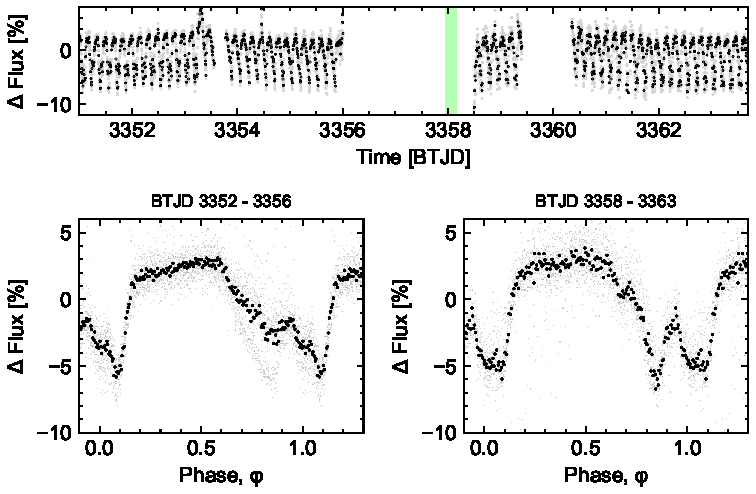
\includegraphics[width=0.99\textwidth]{figures/sf1.pdf}
  \caption{Photometric evolution of TIC 141146667 near the Keck/HIRES observation (green bar). 
  {\bf Panel a}: TESS simple aperture photometry. 
  The main data gaps were caused by scattered light from the Earth
  (BTJD 3356-3358.5) and Moon (BTJD 3359.5-3360.5).
  Raw two minute data are in gray; black time-averages ten minute
  sampling.
  {\bf Panels b,c}: Folded light curve before and after spectroscopy.
  Raw two minute data are in gray; black phase-averages to 100 points
  per cycle.
  During BTJD 3352-3356, a state switch occurred near BTJD 3353,
  in which the dip at $\phi$$\approx$0.8 disappeared.
  While the large eclipse feature remained present before and after
  the HIRES sequence, its photometric shape evolved during the data
  gap.
  }
  \label{fig:fulllc}
\end{figure}

{\it Photometry:} TESS observed TIC~141146667 ($T$=13.3) in Sectors 14,
15, 21, 41, 48, and 75.  Two-minute data were acquired during Sectors
41, 48 (TESS DDT039, PI: Kunimoto), and 75 (TESS Program G06030, PI:
Bouma).  The data from Sectors 14, 15, and 21 had a 30-minute cadence,
which smears sharp features over the $<$4\,hour period (see
\cite{Gunther2022}).  The field is not crowded:  the nearest known
star, TIC~141146666 ($T$=14.5), is 25$''$ from TIC~141146667 and is
photometrically stable in the pixel-level TESS data.

Figure~\ref{fig:fulllc} shows the TESS Sector~75 data acquired near
the epoch of spectroscopy.  The gap in coverage from BTJD
3356.0~-~3358.5 occurred because the Earth was within 25$^\circ$ of
the TESS camera's boresight, yielding high levels of scattered light;
this gap included the Keck/HIRES observation epoch (green bar).  From
BTJD 3359.4~-~3362.0, the Moon then passed within 25$^\circ$ of the
camera's boresight.  Based on the observed level of scattered light in
the optimal TIC~141146667 aperture, we manually masked out times from
3359.40~-~3360.13, and judged the remainder of the data during the
lunar approach to be usable.  Small data gaps from BTJD
3353.55~-~3353.77 and from BTJD 3360.12~-~3360.33 were caused by data
downlinks at the spacecraft's perigee and apogee, respectively.

Figure~\ref{fig:fulllc} shows that a large, complex eclipse
feature was present before and after the HIRES data were
acquired.  From BTJD 3352~-~3356, this eclipse had two sharp local
minima;  the local minimum at $\phi$$\approx$0.8 disappeared following
the flare at BTJD 3353, yielding an eclipse more closely resembling a
long ``V'' than a ``W''.  Similar state changes have previously been
noted and discussed \cite{Stauffer2017,Bouma2024}.  The photometric
shape therefore evolved during the twelve cycles spanning the
3356~-~3358 gap, since the average shape from 3358-3363 more
closely resembles the initial ``W''.



{\it Spectroscopy:}
We observed TIC~141146667 ($V$=16.2) with Keck/HIRES for five hours over
a second-half night spanning 17 February 2024 10:47 to 16:13 (UT).
The star's airmass over this window spanned $z$=1.2-2.2, and we opted
for a fixed 15 minute cadence over the entire sequence, except for a
final 10 minute exposure due to increasing sky brightness at sunrise.
We observed without the iodine cell and used the C2 decker
(0$\farcs$86$\times$14$\farcs$0) in the red instrument configuration,
yielding a spectral resolution $R$$\approx$45{,}0000 ($\delta
v$$\approx$6.7\,\kms; $\delta v / v_{\rm eq}$$\approx$0.05).  We binned
the CCD readout by a factor of three in the spatial dimension, yielding
$\approx$1,000 photons (S/N=33) per pixel in the continuum at 6500\,\AA,
at minimum airmass.  Strong winds contributed to 1\farcs2$\pm$0\farcs2
seeing over the night, but conditions were otherwise favorable.  We
reduced the echelleogram to a one-dimensional spectrum using the
standard techniques of the California Planet Survey \cite{Howard2010}.
Figure~\ref{fig:spec}b shows the result in the vicinity of H$\alpha$
without any additional processing.


\subsection{Stellar Parameters}\phantom{+}
\label{subsec:stparams}

{\it Radial Velocity}---We measured radial velocities of TIC~141146667
from our HIRES spectra using a pipeline that we developed for
rapidly rotating stars.  Our method is based on template-matching
against synthetic spectra produced by the PHOENIX stellar atmosphere
code \cite{Husser2013}.  We used the PHOENIX models with solar
metallicity and alpha element abundances, and calibrated our pipeline
using the standard stars described by \cite{Chubak2012}.  We used
velocity standards spanning spectral types from G2 to M4 (Barnard's
Star), irrespective of rotation rate.  We used \texttt{barycorrpy}
\cite{Kanodia2018} to calculate the velocity corrections due to Earth's
motion around the solar system barycenter and due to Earth's daily
rotation about its axis.  Our analysis code reproduces the systemic
velocities of known velocity standards \cite{Chubak2012} with an RMS of
0.66\,\kms.

For TIC~141146667, we measured the radial velocities using regions near
the K~I (7700\,\AA) resonance line and three TiO bandheads (5160\,\AA,
5450\,\AA, and 5600\,\AA).  We selected these regions because they
provided the best matches between the synthetic and observed spectra.
We then averaged the resulting redshift measurements over each order to
produce the final measurement.  We used the scatter of resulting
velocity measurements between orders to assign the RV uncertainty at
each epoch.  The uncertainty-weighted mean systemic velocity over all
epochs on 17~February~2024 was $\gamma$=0.6$\pm$1.5\,\kms.  The
relative radial velocities about this mean are given in
Table~\ref{tab:rv}.

{\it Viewing Orientation}---We fitted the rotational broadening of the
K~I (7700\,\AA) resonance line using the broadening kernel suggested by
\cite{Gray2008}; taking the mean and standard deviation of the resulting
value over all epochs yielded $v_{\rm eq} \sin i$=138$\pm$8\,\kms,
consistent with the visual line broadening $\Delta
\lambda$$\approx$3\,\AA.  The star's equatorial velocity $v_{\rm eq}$
based on its apparent size and rotation period is 130$\pm$4\,\kms.
While this suggests that the viewing orientation could be nearly
edge-on, the formal constraint is rather weak, with $i$$>$63$^\circ$ at
2$\sigma$ (2.5$^{\rm th}$ percentile of the inclination posterior).

% from calc_max_amplitude_sinusoid_rv_timeseries.py
% from K_to_msini.py, assuming Mstar = 0.18

{\it No Evidence For Binarity}---Any significant periodicity in the
radial velocity time-series is ruled out at the rotation period for
semi-amplitudes above 2.85\,\kms\ (at 3$\sigma$ confidence).  This sets
an upper limit on the mass of any putative companion at the four hour
period of $m \sin i $$<$2.4\,$M_{\rm Jup}$.  Regarding possible
companions at wider separations, the Gaia DR3 renormalized unit weight
error (RUWE), a proxy for the goodness of fit for a single-source
astrometric model to the Gaia astrometry, is 1.23, within the usual
range for apparently single sources.  There are no resolved sources in
the Gaia DR3 point source catalog.  Finally, we checked the TESS light
curve for evidence of secondary photometric periods by subtracting the
mean CPV signal over each sector and performing a phase-dispersion
minimization analysis \cite{Stellingwerf1978,2021zndo...1011188B}.
There were no secondary periods in the TESS data.  Previous work
\cite{Bouma2024} has shown that about 30\% of CPVs show evidence for
excess noise above the Gaia single-source astrometric model, and about
40\% of CPVs show evidence for unresolved binary companions based on the
presence of secondary photometric periods.  This agrees with analyses
showing that multi-periodic low-mass stars are generally unresolved
binaries \cite{Tokovinin2018}.  Overall, the CPV binary fraction seems
consistent with that for field M dwarfs \cite{Winters2019}, pointing to
a weak or non-existent connection between the CPV phenomenon and
(wide) binarity.  For TIC~141146667 specifically, while we find no evidence for
stellar multiplicity, our data are minimally constraining for the
scenario of a low-luminosity companion ($F_1$/$F_2$$\lesssim$0.1) at
with apparent separations below 0$\farcs$1.


\begin{figure}[!t]
  \centering
  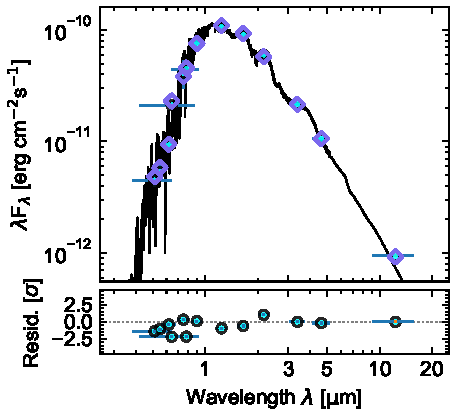
\includegraphics[width=0.7\textwidth]{figures/sf4.pdf}
  \caption{
    Spectral energy distribution of broadband photometric magnitudes
    plotted over the best-fit BT-Settl stellar atmosphere model
    \cite{Allard2012}.  This plot was made from an adaptation of \texttt{astroARIADNE}
    \cite{Vines2022}.  The photometry extends from the Gaia DR3 blue
    passband to WISE W3;  the W4 passband (22 $\mu$m) did not yield
    a confident detection.  This fit yields the star's temperature and
    size.  The lack of excess infrared flux relative to the photospheric
    model sets an upper limit on emission from circumstellar dust.
    }
  \label{fig:sed}
\end{figure}

{\it Effective temperature, radius, mass, and spectral type}---We adopted
the star's effective temperature and radius measured using the spectral
energy distribution (SED) fitting procedure described by
\cite{Bouma2024}.  To summarize, this approach used
\texttt{astroARIADNE} \cite{Vines2022} with the BT-Settl stellar
atmosphere models \cite{Allard2012}, assuming the \cite{Asplund2009}
solar abundances and the \cite{Barber2006} water line lists.  This
approach fitted for the stellar effective temperature, radius,
reddening, surface gravity, metallicity, and distance by comparing the
measured broadband magnitudes against pre-computed model grids.
Specifically, we performed the fit using the broadband magnitudes from
Gaia DR2, APASS, 2MASS, SDSS, and WISE $W1$ and $W2$.  The resulting
best-fit SED is shown in Figure~\ref{fig:sed}.  This method has the most
constraining power for the star's effective temperature (2972 $\pm$
40\,K) and radius (0.42 $\pm$ 0.02\,$R_\odot$); the surface gravity,
metallicity, and reddening are only weakly constrained.  We
determined the star's spectral type to be M5.5Ve by visually comparing
the HIRES spectra against the photometric standards tabulated by
\cite{Bochanski2007}.   This result agrees with the effective
temperature found from the SED fitting \cite{Pecaut2013}.

Given the effective temperature, stellar radius, and age range
(35-150\,Myr) derived below, we then estimated the stellar mass by
interpolating against the PARSEC v1.2S isochrones \cite{Chen2014}.
Specifically, we used the distance metric defined in Equation~8 of
\cite{Bouma2024} to select the model mass closest to a given observed
temperature, radius, and age.  This exercise yielded a mass of
$M_\star$=$0.20\pm0.01$\,$M_\odot$ assuming an age of 35\,Myr, or a mass
of $0.25\pm0.01$\,$M_\odot$ assuming an age of 150\,Myr.  These masses
imply Keplerian corotation radii $R_{\rm cr}/R_\star$=1.75$\pm$0.07 and
$R_{\rm cr}/R_\star$=1.89$\pm$0.07, respectively; this size scale is
relevant because it is theoretically expected to set the inner boundary
at which corotating material might accumulate
(e.g.~\cite{Townsend2005,Daley-Yates2024}).  Our final quoted $M_\star$
and $R_{\rm cr}$ values adopt the average of these extremes and a
quadrature sum of their statistical uncertainties; we caution however
that a more precise age would be needed to resolve the systematic
uncertainties in these parameters.


{\it Age: No Obvious Association Membership}---Previous work
\cite{Bouma2024} has found that over 90\% of CPVs are associated with
known young moving groups based on their positions and kinematics.
TIC~141146667 is in the minority.  We calculated the probability of
TIC~141146667 being part of any of the nearby known groups using
BANYAN\,$\Sigma$ v1.2 \cite{Gagne2018}.  That particular model
classifies it as a field star at $>$99.9\% confidence.  We also searched
the local vicinity of TIC~141146667 for neighbors with similar projected
on-sky velocities using \texttt{comove} \cite{Tofflemire2021}.  This
yielded no strong candidates for co-moving stars with projected
tangential velocities $\Delta v_{\rm T}$$<$5\,\kms\ that share its
isochronal youth.

{\it Age: Isochrones}---The color and absolute magnitude of
TIC~141146667 suggest that it is a pre-main sequence M dwarf, similar to
all other known CPVs \cite{Stauffer2017,Stauffer2021,Bouma2024}.  The
star's proximity ($d$=58\,pc) and its high galactic latitude
($b$=$+$53$^\circ$) yield negligible interstellar reddening along the
line of sight \cite{Green2019}.  Figure~\ref{fig:camd} shows the
location of the star in the color--absolute magnitude diagram (CAMD)
relative to young stellar populations including Upper Scorpius (USco),
IC~2602, and the Pleiades.  To make this diagram, we adopted the USco
members in the $\delta$~Sco and $\sigma$~Sco sub-associations from
\cite{Ratzenbock2023}, and the IC~2602 and Pleiades members from
\cite{Hunt2024}.  We assumed an average $V$-band extinction $A_{\rm
V}$=$\{0.12, 0.11, 0.10\}\,{\rm mag}$ for USco \cite{Pecaut2016},
IC~2602 \cite{Hunt2024}, and the Pleiades \cite{Hunt2024} respectively.
We dereddened the photometry using the extinction coefficients
$k_X\equiv A_X/A_0$ tabulated in \cite{GaiaCollaboration2018}, assuming
that $A_0 = 3.1 E(B-V)$.

Figure~\ref{fig:camd} shows that TIC~141146667 falls between the USco
and Pleiades sequences, while nearly overlapping with IC~2602.  However,
the precision of the implied age is set by the intrinsic scatter of
these calibration sequences; the most luminous stars in the Pleiades of
the same color have a similar absolute magnitude as TIC~141146667.
Previous work \cite{Stauffer2021} has also noted that in the Gaia
passbands, CPVs tend to be photometrically redder and more luminous than
single stars in any given cluster, similar to other rapid rotators.
While this effect complicates any attempt at age inference based on the
Gaia photometry, it suggests that the Pleiades may be a better
comparison population than IC~2602.  Broadly, we take the star's
location in the color--absolute magnitude diagram to suggest age bounds
$t_{\rm CAMD}$$\sim$30-150\,Myr.


{\it Age: Lithium}---The depletion of lithium due to $^7$Li(p,
$\alpha$)$^4$He burning in the cores of low-mass stars has been studied
for over sixty years \cite{Hayashi1963,Bildsten1997,Burke2004}.
\cite{Wood2023} provided an instructive recent overview: an abbreviated
summary is that sufficiently cool and young M dwarfs show the 6707.8\,\AA\
doublet in absorption, $\gtrsim$10\% below their ``continua''.  Unlike
for Sun-like stars, the continuum for M dwarfs is poorly defined due to
their molecular absorption.  We attempted a lithium measurement by
constructing a wavelength-binned and Doppler-corrected TIC~141146667
spectrum, assigning its uncertainties based on the measured scatter
across the five hour dataset.  We then compared this average spectrum
against the nearest matching template from \cite{Bochanski2007}.  The
data show a small depression near the expected lithium wavelength,
potentially consistent with the $\Delta \lambda$$\approx$3\,\AA\ line
broadening.  This feature nominally yields ${\rm EW}_{\rm
Li}$=71$^{+18}_{-13}$\,m\AA, where the statistical uncertainties are
evaluated using a bootstrap resampling technique from the statistical
uncertainties in the spectrum.  However the systematic uncertainties associated
with the continuum normalization are larger, and likely comparable to
the amplitude of the feature; we therefore treat the result of this
measurement as a $2\sigma$ upper limit: ${\rm EW}_{\rm Li}$$<$107\,m\AA.

Despite uncertainties in the details, what can be stated with confidence
is that lithium is not abundant in the spectrum of TIC~141146667.
Figure~\ref{fig:liew_population} compares our upper limit against the
equivalent width measurements reported by \cite{Jeffries2023}
based on the Gaia-ESO spectroscopic survey; Figure~\ref{fig:hirescuts}
shows the associated raw spectra.  If the star were $\lesssim$20\,Myr
old, at its temperature we would expect to see lithium in abundance
($>$400\,m\AA).  Since we do not, we can set an empirical bound on the
lithium-derived age of $t_{\rm Li,emp}$$\gtrsim$20\,Myr.  The
\cite{Feiden2016} lithium isochrones provide a point for theoretical
comparison, and suggest that since $M_{\rm K}$$\approx$6.67\,mag,
$t_{\rm Li,th}$$\gtrsim$35\,Myr is the theoretical age at which
complete depletion occurs in a star with this luminosity (see
e.g.~Figure 7 from \cite{Wood2023}).



\begin{figure}[!t]
  \centering
  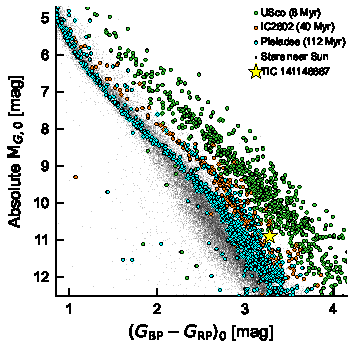
\includegraphics[width=0.7\textwidth]{figures/sf3.pdf}
  \caption{Dereddened Gaia DR3 color vs.~absolute magnitude diagram of
  TIC~141146667 and comparison samples. 
  TIC~141146667 is on the pre-main sequence; stars with the same color
  on the main sequence are $\approx$1.5\,magnitudes
  fainter.  The star's location in this diagram broadly suggests an
  age of 30-150\,Myr.  }
  \label{fig:camd}
\end{figure}


\begin{figure}[!t]
  \centering
  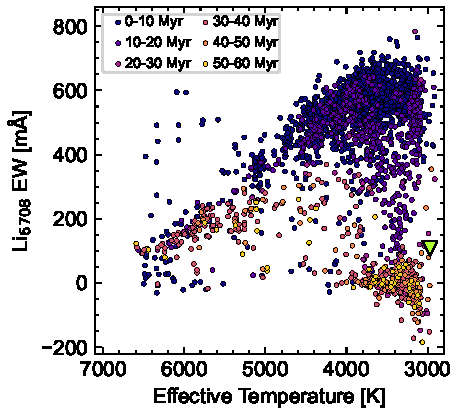
\includegraphics[width=0.7\textwidth]{figures/sf2.pdf}
  \caption{An upper limit on photospheric lithium for TIC~141146667
  (green triangle) yields a lower limit on the star's age of
  $\gtrsim$20\,Myr.  Comparison stars are from the Gaia-ESO survey
  \cite{Jeffries2023}; rich clusters in each age bin include NGC\,2264
  (4.5\,Myr), $\lambda$~Ori (8.7\,Myr), ${\rm \gamma}^2$\,Vel
  (16.4\,Myr), NGC\,2547 (35.0\,Myr), IC\,2602 and IC\,2391 (42.0\,Myr),
  and NGC\,2451A (50.0\,Myr). }
  \label{fig:liew_population}
\end{figure}


{\it Age: Summary}---The main indicators for the youth of
TIC~141146667 are {\it i)} that it is a complex periodic variable, and
{\it ii)} that it is 1.5 magnitudes brighter than main sequence stars
of the same color, while showing no indicators for binarity.  The
first item constitutes evidence for youth since all known CPVs are
$\lesssim$200\,Myr \cite{Bouma2024}.  The reference sequences for the
Pleiades (112\,Myr, \cite{Dahm2015}) show a few stars of equal
luminosity and the same temperature, suggesting a photometric
isochronal age upper limit $\lesssim$150\,Myr.  The weak lithium
absorption suggests an age of at least 20\,Myr based on an empirical
comparison using Gaia-ESO spectra, or at least 35\,Myr based on the
\cite{Feiden2016} isochrones.  These considerations yield our adopted
age range of 150\,Myr.



{\it Upper and Low Bounds on Dust}---An upper limit on the amount of
hot dust follows from the lack of an infrared excess.  A lower limit
follows if one assumes that most of the broadband optical depth comes
from dust absorption and scattering, rather than any radiative
processes associated with the plasma.

Regarding the upper limit, Figure~\ref{fig:sed} shows the SED.  While
AllWISE \cite{Cutri2014} yielded a confident W3 detection
(9.8$\sigma$), the W4 extraction yielded only a marginal indication
(1.7$\sigma$) of detectable flux.  Similar to other CPVs
\cite{Stauffer2017,Bouma2024}, the photometric uncertainties from WISE
W1 and W2 allow at most a $\lesssim$2\% excess at 3-5\,$\mu$m relative
to the stellar photosphere, and a $\lesssim$5\% excess at 10\,$\mu$m
(W3).  To estimate the implied mass bound, we assume a dust
temperature $T_{\rm d}$=1500\,K, typical for dust near the star (see
\cite{Zhan2019} for discussion regarding dust sublimation).  We then
treat emission from the dust and the star as Planck functions, and
require $L_{\rm d} < f L_\star$, where the factor $f$ is set by
photometric precision of WISE and $L_{\rm d}$ is the bolometric dust
luminosity.  Given the reported uncertainties, we numerically find
$f<6\cdot$10$^{-3}$.  From the Stefan-Boltzmann law we can then write
$A_{\rm d} < f (T_\star / T_{\rm d})^4 Q_{\rm em}^{-1} (4\pi
R_\star)^2$, for $A_{\rm d}$ the total emitting surface area of the
dust, and $Q_{\rm em}$ is an emission efficiency parameter.
Converting this constraint to a dust mass requires an assumption
regarding the grain properties.  We assume a grain density $\rho_{\rm
d}$=3\,g\,cm$^{-3}$ typical for silicate grains, a fixed grain size
$a$=1\,$\mu$m \cite{Tanimoto2020,Gunther2022,Koen2023}, and no
self-absorption.  This enables the assumption that $A_{\rm d} = N \pi
a^2$, for $N$ the total number of dust grains.  This in turn yields an
upper limit on the dust mass of
\begin{equation}
  M_{\rm dust} \lesssim 4 \cdot 10^{17}\, {\rm g}\ 
  \left( \frac{f}{6\cdot10^{-3}} \right)
  \left( \frac{T_\star}{3000\,{\rm K}} \frac{1500\,{\rm K}}{T_{\rm d}} \right)^4
  \left( \frac{Q_{\rm em}}{1} \right)^{-1}
  \left( \frac{R_\star}{0.4\,R_\odot} \right)^2
  \left( \frac{a}{1\,\mathrm{\mu m}} \right)
  \left( \frac{\rho_{\rm d}}{3\,\mathrm{g\,cm^{-3}}} \right).
\end{equation}

The analogous lower limit follows from requiring the optical depth
from absorption and scattering $\tau$ to be at least unity.  The
optical depth can be written $\tau = n \sigma \ell = N \sigma$, where
$\sigma$ is the cross-section, $n$ is the number density, $\ell$ is
the path length, and $N$ is the column density.  For spherical dust
grains in the optical, $\sigma = Q_{\rm ext} \pi a^2$, where $Q_{\rm
ext}$ is the extinction efficiency parameter, tabulated e.g.~by
\cite{Croll2014} in their Figure 13.  \cite{Sanderson2023} calculated
the relevant cloud mass scaling assuming a spherical dust clump of
size $r$, and they estimated
\begin{equation}
  M_{\rm dust} \gtrsim 2 \cdot 10^{15}\, {\rm g}\ 
  \left( \frac{\tau}{1} \right)
  \left( \frac{Q_{\rm ext}}{3} \right)^{-1}
  \left( \frac{r}{0.1\,R_\star} \frac{R_\star}{0.4\,R_\odot} \right)^2
  \left( \frac{a}{1\,\mathrm{\mu m}} \right)
  \left( \frac{\rho_{\rm d}}{3\,\mathrm{g\,cm^{-3}}} \right).
\end{equation}

Three relevant objects for comparison to these limits include solar
prominences, planetesimals, and comets.
Prominences of the Sun typically have gas masses
of order $10^{14}$\,g-$10^{16}$\,g \cite{VialEngvold2015}.
A planetesimal of mass $\approx$10$^{15}$\,g with a bulk density of
1\,g\,cm$^{-3}$ would have a diameter of order one kilometer.
Halley's comet has a mass of order $10^{17}$\,g \cite{Rickman1989}, of
which $\sim$$10^{14}$\,g is shed per orbit, most of which inspirals
toward the Sun due to Poynting-Robertson drag.
Broadly, these calculations suggest that if dust is responsible for
the broadband variability of CPVs, it would need to be concentrated in
clumps with masses in the range of $10^{15}$-$10^{17}$\,g.



\subsection{Spectroscopic Variability}\phantom{+}

\begin{figure}[!t]
  \centering
  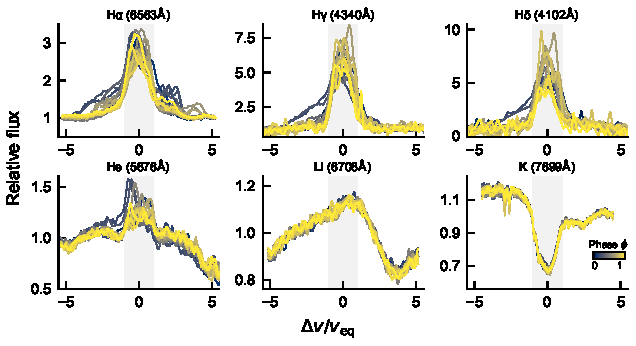
\includegraphics[width=\textwidth]{figures/sf5.pdf}
  \caption{Time evolution of select regions in the Keck/HIRES
  spectra from 17 February 2025.
  The spectra have been smoothed with a Gaussian filter.
  The horizontal axis shows the relative velocity centered on each
  line's rest wavelength, normalized by the stellar equatorial
  velocity.  
  H$\alpha$ is the only Balmer line to show periodic variability of
  the form seen in Figure~\ref{fig:spec}.
  The He 5876\,\AA\ line shows a time-dynamic blueshift that 
  differs from the Balmer lines.
  Li 6708\,\AA\ shows no obvious absorption.
  }
  \label{fig:hirescuts}
\end{figure}

Figure~\ref{fig:hirescuts} shows a few regions of interest in the HIRES
spectra, which cover 3650-7960\,\AA.
Higher order Balmer lines including H$\gamma$ and H$\delta$ (the
$n=5\rightarrow2$ and $n=6\rightarrow2$ transitions respectively) do
show some variability outside the line core.
However, this variability is not clearly periodic in the
same manner as the emission seen in H$\alpha$.
This could be because there are insufficient hydrogen ions in the
relevant excited states, or due to the lower precision of the spectra
in these bluer regions.
The Ca HK doublet for instance is also detectable in emission, however
the continuum near it is not.
Chromospheric emission lines in the magnesium triplet order are
also detectable, but sufficiently blended to be rendered unusable.

One notable feature is that H$\alpha$, H$\gamma$, H$\delta$, and He
5876\,\AA\ all show a blue excess at $\phi$$\approx$0.2.  At the same
epoch, only H$\alpha$ clearly shows a resolved red excess as well,
although $H\gamma$ and H$\delta$ are broader at this time.  Given the
sudden rise of this emission in $<$15\,minutes, and the association
between He 5876\,\AA\ and stellar outflows at high excitation energy,
this component of the spectra might be more easily associated with a
flare than with a stable, periodic component.

Finally, the Li\,\textsc{I} 6708\,\AA\ doublet, which shows no obvious
absorption, as well as the broad K\,\textsc{I} 7699\,\AA\ resonance
line are both shown in Figure~\ref{fig:hirescuts}.  In the latter,
narrow telluric absorption features overlap the blue wing of the line.
Neither of these regions shows any notable variability.


\subsection{Modeling the Emitting Clump}
\label{subsec:model}

The physical conditions inside the circumstellar plasma clumps, in
particular the hydrogen number density, plasma temperature, ionization
fraction, and magnetic field strength can all be estimated using the
available data.
We caution that the following estimates are coarse: detailed
considerations of radiative transfer and detailed balance are a
worthwhile topic for future work, but are beyond our immediate scope.

Circumstellar H$\alpha$ emission might be sourced either from
scattering of stellar H$\alpha$ photons, or from recombination.  We
neglect scattering because we see the amplitude of the circumstellar
emission to vary by a factor of $\approx$5, which is not mirrored in
the chromospheric line core.  The volume emissivity under case B
recombination (in which Lyman-series photons are trapped by high
optical depth, so that recombinations cascade through H$\alpha$ and
other Balmer lines) can be written as
\begin{equation}
  j_{\rm H\alpha} = n_{\rm e} n_{\rm p} \alpha^{\rm eff}_{\rm H\alpha}(T) h \nu_{\rm H\alpha},
\end{equation}
where $n_{\rm e}$ and $n_{\rm p}$ are the electron and proton densities,
and $\alpha^{\rm eff}_{\rm H\alpha}(T)$ is the effective recombination
coefficient, i.e.\ the number of recombinations per unit volume, per
unit time.
For hydrogen with temperatures between 1,000 and 10,000\,K with
densities $n_{\rm H}$$\sim$10$^{10}$\,cm$^{-3}$,
$\alpha^{\rm eff}_{\rm H\alpha}$ is typically on the order of $10^{-12}$ to
$10^{-13}$\,cm$^3$\,s$^{-1}$ \cite{Hummer1987}.
Neglecting the effects of atoms other than hydrogen, we can assume
an ionization fraction $x$, such that $n_{\rm e} = n_{\rm p} = x
n_{\rm H}$, for $n_{\rm H}$ the hydrogen number density.  Let $L_{\rm
H\alpha} = j_{\rm H\alpha} V$, for $V$ the volume of the emitting
hydrogen.
The luminosity of circumstellar hydrogen emission, $L_{\rm H\alpha}$,
is an observable: our SED fitting routine yields
$L_\star$$\approx$0.012\,$L_\odot$, which gives
$L_{\rm H\alpha},\star$$\approx$1.0$\times$$10^{28}$erg\,s$^{-1}$, and
the luminosity of the clump $L_{\rm H\alpha}$ is of order one tenth
that of the star.
Assuming an emitting sphere of radius $r$, we can write
\begin{equation}
  n_H = \frac{1}{x}
  \left( 
    \frac{L_{\rm H\alpha}}{ \alpha^{\rm eff}_{\rm H\alpha}(T) h \nu_{\rm H\alpha} V }
  \right)^{1/2}.
\end{equation}
Taking nominal parameters of $r = 0.1 R_\star$, $x=1/2$, and
$\alpha^{\rm eff}_{\rm H\alpha}$=$10^{-13}$\,cm$^3$\,s$^{-1}$,
we find $n_{\rm H}\approx 5\times10^{11}$\,cm$^{-3}$.
Assuming a uniform density clump, this yields $M_{\rm H}\approx
8\times10^{16}$\,g.
A constraint on the magnetic field strength at the site of the clump
follows from the requirement that the magnetic pressure exceed the
thermal pressure, $B^2 / 8\pi > n_{\rm H} k T$.
Although we do not know the plasma temperature,
if it were significantly outside the range of
1,000 and 10,000\,K,
we would either full ionize the hydrogen, or not ionized enough of it.
We can therefore estimate
\begin{equation}
  B \gtrsim 3\,{\rm G}
  \left(
  \frac{n_{\rm H}}{5\times10^{11}\,{\rm cm}^{-3}}
  \frac{T}{5000\,{\rm K}}
  \right).
\end{equation}
Given that the average surface magnetic field strengths of low-mass
stars have been measured to span hundreds to thousands of Gauss
\cite{Kochukhov2021}, this bound is easily met.

%%%%%%%%%%%%%%%%%%%%%%%%
% Supplementary Tables %
%%%%%%%%%%%%%%%%%%%%%%%%

% TEMPLATE: IRAS041
%
\begin{table}
    \centering
    \begin{tabular}{lcr}
    \hline 
    \hline
    Parameter & Host & Source \\
    \hline 
    \multicolumn{3}{c}{Identifiers} \\
    \hline
    TIC & 141146667 & TESS \\
    Gaia & 860453786736413568 & Gaia\ DR3 \\
    %2MASS & J04154278+2909597 & J04154269+2909558 & 2MASS \\
    %ALLWISE & J041542.77+290959.5 & ... & ALLWISE\\
    \hline
    \multicolumn{3}{c}{Astrometry \& Radial Velocity} \\ 
    \hline
    $\alpha_{2000}$ & 11:05:15.09   & Gaia\ DR3 \\
    $\delta_{2000}$ & +59 15 05.57  & Gaia\ DR3 \\
    $\mu_{\alpha}$ (mas yr$^{-1}$ ) & -73.933 $\pm$ 0.022 & Gaia\ DR3 \\
    $\mu_{\delta}$ (mas yr$^{-1}$ ) &  32.262 $\pm$ 0.024 & Gaia\ DR3 \\
    $\pi$ (mas)                     &  17.324 $\pm$ 0.025 & Gaia\ DR3 \\
    RUWE                            &  1.23               & Gaia\ DR3 \\
    RV (\kms)                       & 0.61 $\pm$ 1.47     & HIRES \\
    \hline
    \multicolumn{3}{c}{Photometry} \\
    \hline
    $TESS$ (mag)                    & 13.283 $\pm$ 0.010 & TIC8\     \\
    $G$ (mag)                       & 14.701 $\pm$ 0.002 & Gaia\ DR3 \\
    $G_{\rm BP}$ (mag)              & 16.664 $\pm$ 0.008 & Gaia\ DR3 \\
    $G_{\rm RP}$ (mag)              & 13.398 $\pm$ 0.006 & Gaia\ DR3 \\
    $G_{\rm BP}$-$G_{\rm RP}$ (mag) &  3.276 $\pm$ 0.010 & Gaia\ DR3 \\
    $J$ (mag)                       & 11.401 $\pm$ 0.022 & 2MASS     \\
    $H$ (mag)                       & 10.793 $\pm$ 0.021 & 2MASS     \\
    $K_s$ (mag)                     & 10.473 $\pm$ 0.016 & 2MASS     \\
    $W1$ (mag)                      & 10.276 $\pm$ 0.023 & ALLWISE   \\ % Cutri+2013 II/328/allwise
    $W2$ (mag)                      & 10.070 $\pm$ 0.020 & ALLWISE   \\
    $W3$ (mag)                      &  9.838 $\pm$ 0.045 & ALLWISE   \\
    %$W4$ (mag)                      &  8.392 $\pm$ NOUNC & ALLWISE \\
	  %
    %TODO: eROSITA?  ROSAT is an emitter.  GALEX detection.
    % Ofek+2011 1.4Ghz emitter.  Helfand+2015 ditto.  Bruzewski+2021.
    %\hline
    %\multicolumn{3}{c}{Kinematics and Position} \\
    %\hline
    %$RV$ (\kms) & 0.61 $\pm$ 1.47 & HIRES \\
    %$U$ (\kms)  & & \\
    %$V$ (\kms)  & & \\
    %$W$ (\kms)  & & \\
    %$X$ (pc)    & -28.4 & \\
    %$Y$ (pc)    &  19.8 & \\
    %$Z$ (pc)    &  67.0 & \\
    \hline
    \multicolumn{3}{c}{Physical Properties} \\
    \hline
    $T_{eff}$ (K) & 2972 $\pm$ 40 & \cite{Bouma2024} SED fit\\
    $R_\star$ ($R_{\odot}$) & 0.42 $\pm$ 0.02 & \cite{Bouma2024} SED fit \\
    $P_{\rm rot}$ (hours) & $3.930\pm 0.001$ & TESS \\ 
    $v_{\rm eq}$ (\kms)  &  130$\pm$4  & Derived \\
    $v_{\rm eq} \sin i_\star$(km s$^{-1}$) & $138 \pm 8$ & HIRES \\
    $i_\star$($^\circ$) & $>$63 & Derived \\
    $A_V$ (mag) & 0 & \cite{Green2019} \\
    %$F_{bol}$ (erg cm$^{-2}$ s$^{-1}$ ) & todo & This work\\
    %$L_\star$ ($L_{\odot}$)  & todo & This work\\
    $M_\star$ ($M_{\odot}$)  & 0.22 $\pm$ 0.02  & PARSEC \cite{Chen2014}\\
    ${\rm EW}_{\rm Li}$ (m\AA) & $<$107 & HIRES (2$\sigma$)\\
    $t_{\rm CAMD}$ (Myr) & 30-150 &  Gaia DR3 \\
    $t_{\rm Li,emp}$ (Myr) & $>$20 &  HIRES, \cite{Jeffries2023} \\
    $t_{\rm Li,th}$ (Myr) & $>$35 &  HIRES, \cite{Feiden2016} \\
    $t_{\rm adopted}$ (Myr) & 35-150 &  -- \\
    \hline
    \end{tabular}
		\caption{Properties of \starname.  References:
    Gaia DR3 \cite{GaiaDR3}, TESS \cite{Ricker2015},
    TIC8 \cite{Stassun2019}, 2MASS \cite{Skrutskie2006}, ALLWISE
    \cite{Cutri2014}.}
    \label{tab:stparams}
\end{table}


\begin{table}
  \centering
  \begin{tabular}{lcr}
  %\setlength{\tabcolsep}{2pt}
  \hline 
  \hline 
  Time [JD$_{\rm UTC}$] & RV (\kms) & $\sigma_{\rm RV}$ (\kms) \\
  % from tables/tab_TIC141146667_rel_rv.tex
  \hline 
  60357.450329 & 2.73 & 5.86 \\
  60357.461255 & -4.40 & 2.37 \\
  60357.472181 & -0.19 & 2.64 \\
  60357.483109 & 3.84 & 2.87 \\
  60357.494030 & 7.53 & 7.53 \\
  60357.504949 & -1.98 & 1.44 \\
  60357.515873 & 1.02 & 1.21 \\
  60357.526794 & 0.64 & 7.03 \\
  60357.537717 & -2.91 & 2.71 \\
  60357.548639 & 8.93 & 6.75 \\
  60357.559566 & 5.95 & 8.84 \\
  60357.570487 & -2.25 & 3.06 \\
  60357.581408 & 1.84 & 1.34 \\
  60357.592330 & 2.41 & 8.24 \\
  60357.603251 & -7.04 & 3.94 \\
  60357.614172 & -2.24 & 3.07 \\
  60357.625095 & -2.83 & 7.55 \\
  60357.636019 & -0.59 & 2.26 \\
  60357.646940 & 1.84 & 2.91 \\
  60357.657861 & 4.54 & 3.95 \\
  60357.668781 & 6.21 & 12.14 \\
  \hline
  \end{tabular}
  \caption{TIC~141146667 radial velocities relative to the systemic velocity.}
  \label{tab:rv}
\end{table}



\end{methods}

\bibliography{cpvbib.bib} % common bib file
\bibliographystyle{naturemagfixed}   


\begin{addendum}

\item[Acknowledgments]
  % convos w/
  % M.~Jardine. (line core sum, explaining flux tubes)
  % A Weinberger (dissolving rocks)
  % L Hillenbrand (general?)
  % line profile analysis by B.~Tofflemire.
  % CPS group for reduction support.
  The author thanks X, Y, Z.
  L.G.B. was suported by...
	Acknowledge TESS...
  Acknowledge use of IRSA.


%TC:ignore
%% Author Contribution
\item[Author Contributions] ...
%TC:endignore

\item[Data Availability] ...

\item[Competing Interests] The authors declare that they have no competing
financial interests.
 
\item[Correspondence] Correspondence and requests for materials should be
addressed to ...
 
\item[Code availability] We provide access to a GitHub repository including all
code created for the analysis of this project that is not already publicly
available.

\end{addendum}



\end{document}


